% Dubins_math.tex: the formulas of Dubins_TSP_New_Implementation_claude/dubins_path.py,
% in the notation and style of Section 0.13 of Dubins_TSP.pdf.
%
% Build from this folder (needs the figures from make_figures.py):
%   python make_figures.py
%   python check_formulas.py      # the agreement with the code quoted in the text
%   pdflatex Dubins_math.tex && pdflatex Dubins_math.tex
%   mv Dubins_math.pdf ..
\documentclass[10pt]{article}
\usepackage[letterpaper,margin=1in]{geometry}
\usepackage{amsmath,amssymb}
\usepackage{graphicx}
\usepackage{booktabs}
\usepackage{array}
\usepackage{tabularx}
\usepackage{float}
\usepackage[font=small,labelfont=bf]{caption}
\usepackage[hidelinks]{hyperref}

\newcommand{\code}[1]{\texttt{#1}}
\newcommand{\Stan}{S_{\tan}}
\newcommand{\Spath}{S_{\mathrm{path}}}
\newcommand{\xtraj}{x_{\mathrm{trajectory}}}
\newcommand{\ytraj}{y_{\mathrm{trajectory}}}
\newcommand{\straj}{s_{\mathrm{trajectory}}}
\newcommand{\dcoci}{d_{co,ci}}
\newcommand{\Turn}{\Delta}
\newcommand{\TT}[1]{\mathrm{#1}}
\newcommand{\lb}{\char`\{}
\newcommand{\rb}{\char`\}}

\begin{document}

\begin{center}
  {\LARGE Dubins Path: the Mathematics of \code{dubins\_path.py}}\\[1.2em]
  {\large November 2026}
\end{center}
\vspace{1em}

This note states every formula that \code{dubins\_path.py} (in \code{Dubins\_TSP\_New\_Implementation\_claude/})
computes, in the notation of Section~0.13 of \code{Dubins\_TSP.pdf}. Beside each symbol is the name it has in the
code, and each section names the functions it describes, so every formula can be found in the program. All closed
forms below were checked against the code on 20\,000 random pairs of poses ($R = 5$\,m, points in a 40\,m square),
which gave 74\,236 CSC and 18\,450 CCC paths: they agree to within $10^{-13}$\,m.

\section{Vehicle Model and Notation}

Given two positions
\[
  (x_1, y_1, \psi_1), \qquad (x_2, y_2, \psi_2),
\]
we are to find a Dubins path of minimum turn radius $R$ from the first to the second. The mobile sink moves
forward only, at constant speed $v$:
\begin{equation}
  \begin{bmatrix} \dot{x} \\ \dot{y} \\ \dot{\psi} \end{bmatrix}
  = v \begin{bmatrix} \cos\psi \\ \sin\psi \\ \frac{\alpha}{R} \end{bmatrix},
  \qquad \alpha \in [-1, 1].
  \label{eq:kinematics}
\end{equation}
This is eq.~(21) of the paper, with the heading written $\psi$ as in Section~0.13. Headings are in radians,
measured anticlockwise from the $x$ axis. A Dubins path uses only the three extreme controls: $\alpha = 1$ (a left
arc of radius $R$), $\alpha = -1$ (a right arc of radius $R$) and $\alpha = 0$ (a straight line). The direction of
an arc is
\begin{equation}
  \sigma = \begin{cases} +1 & \text{left turn (anticlockwise)},\\ -1 & \text{right turn (clockwise)}, \end{cases}
  \label{eq:sigma}
\end{equation}
which is \code{SIGMA = \lb"L": 1, "R": -1\rb} in the code. A path has three parts, and its turn type
(\code{turnType}) is one of the six words
\[
  \text{LSL}, \quad \text{RSR}, \quad \text{LSR}, \quad \text{RSL}, \quad \text{RLR}, \quad \text{LRL}
\]
(\code{TURN\_TYPES}), where L is a left arc, R a right arc and S a straight line. $\sigma_1$ is the direction of the
first letter and $\sigma_2$ that of the last. In a CSC path the middle part is straight. In a CCC path
$\sigma_1 = \sigma_2$ and the middle arc turns the other way, with direction $-\sigma_1$.

Table~\ref{tab:notation} lists the symbols. A centre of a circle is always written with a digit,
$(x_{c1}, y_{c1})$, $(x_{c2}, y_{c2})$ or $(x_{c3}, y_{c3})$, so $(x_{ci}, y_{ci})$ always means the cut-in point.

\begin{table}[t]
\centering
\small
\caption{Symbols and their names in \code{dubins\_path.py}.}
\label{tab:notation}
\begin{tabularx}{\textwidth}{@{}l l >{\raggedright\arraybackslash}X@{}}
\toprule
Symbol & Code & Meaning \\
\midrule
$x_1, y_1, \psi_1$ & \code{x1, y1, psi1} & start point and start heading \\
$x_2, y_2, \psi_2$ & \code{x2, y2, psi2} & end point and end heading \\
$R$ & \code{R} & minimum turning radius (5\,m with the defaults of \code{config.py}) \\
$\sigma_1, \sigma_2$ & \code{sigma1, sigma2} & direction of the first and the last arc, eq.~\eqref{eq:sigma} \\
$\hat{u}_1, u_2, \hat{u}_3$ & \code{u\_vec1, u\_vec2, u\_vec3} & vectors of the turn-type rule \\
$cp_1, cp_2$ & \code{cp1, cp2} & cross products of the turn-type rule \\
$(x_{c1}, y_{c1}), (x_{c2}, y_{c2})$ & \code{xc1, yc1, xc2, yc2} & centres of the first and the last circle \\
$(x_{c3}, y_{c3})$ & \code{xc3, yc3} & centre of the middle circle of a CCC path \\
$\Stan$ & \code{Stan} & distance between $(x_{c1}, y_{c1})$ and $(x_{c2}, y_{c2})$ \\
$\psi_L$ & \code{psiL} & direction of the line from the first to the last centre \\
$\psi_D$ & \code{psiD} & heading of the straight part (the cut-out angle $\psi_d$ of Section~0.13) \\
$\beta$ & \code{cutOutAngle} & angle between the straight part and the line of centres (LSR, RSL) \\
$\theta$ & \code{theta} & angle at $(x_{c1}, y_{c1})$ between the lines to the other two centres (CCC) \\
$\psi_{co}, \psi_{ci}$ & \code{psiCO, psiCI} & headings at the cut-out and the cut-in point (CCC) \\
$(x_{co}, y_{co})$ & \code{xco, yco} & cut-out point, where the first arc ends \\
$(x_{ci}, y_{ci})$ & \code{xci, yci} & cut-in point, where the last arc starts \\
$\hat{u}, \dcoci$ & \code{u\_hat, dist} & direction and length of the straight part \\
$S_1, S_3, S_2$ & \code{S1, S3, S2} & lengths of the first, the middle (CCC) and the last arc \\
$\Spath$ & \code{pathDistance} & total length of the path \\
$\psi_T$ & \code{psiT} & heading at the end of the part computed so far \\
$\Delta s$ & \code{step} & spacing of the points along the path (\code{p["ds"]} = 0.25\,m) \\
$\xtraj, \ytraj$ & \code{xtrajectory, ytrajectory} & the points of the path \\
$\straj$ & \code{strajectory} & distance along the path of each point \\
\bottomrule
\end{tabularx}
\end{table}

\section{Basic Geometry}

\paragraph{Centre of a turning circle} (\code{returnCircleCenter}). The circle of direction $\sigma$ that passes
through $(x, y)$ with heading $\psi$ has its centre a distance $R$ to the left ($\sigma = 1$) or to the right
($\sigma = -1$) of the heading:
\begin{equation}
  (x_c, y_c) = \Bigl( x + R \cos\bigl(\psi + \tfrac{\pi}{2}\sigma\bigr),\;
                      y + R \sin\bigl(\psi + \tfrac{\pi}{2}\sigma\bigr) \Bigr).
  \label{eq:centre}
\end{equation}
The first circle uses $(x_1, y_1, \psi_1, \sigma_1)$ and gives $(x_{c1}, y_{c1})$. The last circle uses
$(x_2, y_2, \psi_2, \sigma_2)$ and gives $(x_{c2}, y_{c2})$.

\paragraph{Distance and direction between the centres} (\code{distance}, \code{atan2}).
\begin{equation}
  \Stan = \sqrt{(x_{c2} - x_{c1})^2 + (y_{c2} - y_{c1})^2},
  \label{eq:stan}
\end{equation}
\begin{equation}
  \psi_L = \operatorname{atan2}(y_{c2} - y_{c1},\; x_{c2} - x_{c1}).
  \label{eq:psiL}
\end{equation}
$\operatorname{atan2}$ gives the angle in $(-\pi, \pi]$ in the correct quadrant and divides by nothing, so it is
defined even when $x_{c2} = x_{c1}$.

\paragraph{Turning angle} (\code{turnAngle}). On a circle of direction $\sigma$ the heading can only change in the
direction $\sigma$. To go from heading $\psi_a$ to heading $\psi_b$ the sink therefore turns through
\begin{equation}
  \Turn_\sigma(\psi_a, \psi_b) = \bigl[\sigma(\psi_b - \psi_a)\bigr] \bmod 2\pi, \qquad
  0 \le \Turn_\sigma(\psi_a, \psi_b) < 2\pi,
  \label{eq:turn}
\end{equation}
and drives an arc of length $R\,\Turn_\sigma(\psi_a, \psi_b)$. Here $a \bmod 2\pi = a - 2\pi \lfloor a / 2\pi \rfloor$
is never negative, so no check is needed for a heading passing $\pi$ or $-\pi$. To stop a rounding error from turning
``no turn'' into a full circle, the code sets
\begin{equation}
  \Turn_\sigma(\psi_a, \psi_b) = 0 \quad \text{if} \quad \Turn_\sigma(\psi_a, \psi_b) > 2\pi - 10^{-6}.
  \label{eq:turn-guard}
\end{equation}
Headings can be off by about $10^{-7}$\,rad when $\Stan$ is almost exactly $2R$, because $\sin^{-1}$ is very
sensitive near 1.

\paragraph{Driving along an arc} (\code{pointsOnArc}). A sink that starts at $(x, y)$ with heading $\psi$ and drives
$s$ metres on the circle of direction $\sigma$, whose centre $(x_c, y_c)$ is given by eq.~\eqref{eq:centre}, is at
\begin{equation}
  \begin{bmatrix} x(s) \\ y(s) \end{bmatrix} =
  \begin{bmatrix} \cos\alpha & -\sigma\sin\alpha \\ \sigma\sin\alpha & \cos\alpha \end{bmatrix}
  \begin{bmatrix} x - x_c \\ y - y_c \end{bmatrix} +
  \begin{bmatrix} x_c \\ y_c \end{bmatrix},
  \qquad \alpha = \frac{s}{R},
  \label{eq:arc}
\end{equation}
with heading
\begin{equation}
  \psi(s) = \psi + \sigma\,\frac{s}{R}.
  \label{eq:arc-heading}
\end{equation}
Eq.~\eqref{eq:arc} is the rotation matrix of Section~0.13.1 with the exact angle $s/R$ in place of the step
$i\,\Delta\psi$.

\section{The Turn-Type Rule of Section 0.13}
\label{sec:rule}

These formulas are in \code{findTurnType}, \code{findCSCTurnType} and \code{findCCCTurnType}. The path uses them
only when \code{dubins\_method} is \code{"pdf"} in \code{config.py}. Define
\begin{equation}
  \hat{u}_1 = \begin{bmatrix} \cos\psi_1 \\ \sin\psi_1 \end{bmatrix}, \qquad
  u_2 = \begin{bmatrix} x_2 - x_1 \\ y_2 - y_1 \end{bmatrix}, \qquad
  \hat{u}_3 = \begin{bmatrix} \cos\psi_2 \\ \sin\psi_2 \end{bmatrix}.
  \label{eq:rule-vectors}
\end{equation}
Only the signs of the cross products are used, so $u_2$ is not divided by its length; this also avoids dividing by
zero when the two points coincide. The cross products are
\begin{equation}
  \begin{aligned}
  cp_1 &= \hat{u}_1 \times u_2 = \cos\psi_1\,(y_2 - y_1) - \sin\psi_1\,(x_2 - x_1),\\
  cp_2 &= u_2 \times \hat{u}_3 = (x_2 - x_1)\sin\psi_2 - (y_2 - y_1)\cos\psi_2 .
  \end{aligned}
  \label{eq:cp}
\end{equation}
$cp_1 > 0$ when the end point lies to the left of the start heading, and $cp_2 > 0$ when the end heading points to
the left of $u_2$. The CSC turn type is determined as follows:
\begin{equation}
  \begin{cases}
    cp_1 \le 0,\ cp_2 \ge 0 & \Rightarrow \text{turn type} = \TT{RSL}, \quad \sigma_1 = -1,\ \sigma_2 = 1,\\
    cp_1 \le 0,\ cp_2 < 0   & \Rightarrow \text{turn type} = \TT{RSR}, \quad \sigma_1 = -1,\ \sigma_2 = -1,\\
    cp_1 > 0,\  cp_2 < 0    & \Rightarrow \text{turn type} = \TT{LSR}, \quad \sigma_1 = 1,\ \sigma_2 = -1,\\
    cp_1 > 0,\  cp_2 \ge 0  & \Rightarrow \text{turn type} = \TT{LSL}, \quad \sigma_1 = 1,\ \sigma_2 = 1.
  \end{cases}
  \label{eq:rule}
\end{equation}
The case $cp_2 = 0$, where the end heading lies along $u_2$, is treated like $cp_2 > 0$. Then the centres follow
from eq.~\eqref{eq:centre} with these $\sigma_1, \sigma_2$, and $\Stan$ from eq.~\eqref{eq:stan}. Only RSR and LSL can
become CCC curves:
\begin{equation}
  \text{if } 2R \le \Stan < 3R: \qquad
  \TT{RSR} \Rightarrow \TT{RLR} \ (\sigma_1 = \sigma_2 = -1), \qquad
  \TT{LSL} \Rightarrow \TT{LRL} \ (\sigma_1 = \sigma_2 = 1).
  \label{eq:rule-ccc}
\end{equation}
LSR and RSL stay CSC curves for every $\Stan$. The turn type chosen this way may not exist for the given poses (LSR
or RSL with $\Stan < 2R$); Section~\ref{sec:choose} says what is done then.

\section{Lengths of the Three Parts}
\label{sec:lengths}

These formulas (\code{calculateCSCLengths}, \code{calculateCCCLengths}) take one turn type and return the lengths of
its three parts. Each turn type has its own $\sigma_1$ and $\sigma_2$, and therefore its own centres, $\Stan$ and
$\psi_L$ from eqs.~\eqref{eq:centre}--\eqref{eq:psiL}. The functions accept arrays of headings as well as single
numbers, so one call gives the lengths for many start and end headings at once.

\subsection{CSC Paths}

\begin{figure}[!htb]
  \centering
  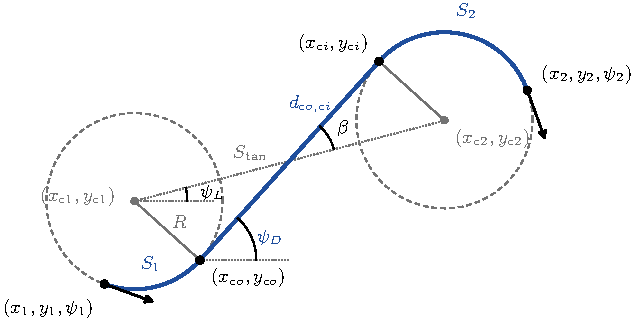
\includegraphics[width=0.74\textwidth]{fig_csc.pdf}
  \caption{An LSR path, drawn by \code{dubins\_path.py} from $(0, 0, -20^\circ)$ to $(24, 11, -70^\circ)$ with
  $R = 5$\,m. The circles' centres are $\Stan = 18.18$\,m apart in direction $\psi_L = 14.6^\circ$. The straight
  part crosses the line of centres at its midpoint, at the angle $\beta = \sin^{-1}(2R/\Stan) = 33.4^\circ$, so its
  heading is $\psi_D = \psi_L + \beta = 48.0^\circ$. The lengths are $S_1 = 5.93$, $\dcoci = 15.18$ and
  $S_2 = 10.30$\,m. Here LSR is both the shortest path and the choice of the rule of Section~0.13.}
  \label{fig:csc}
\end{figure}

Where the straight part, with heading $\psi_D$, touches circle $k$, the centre of that circle lies a distance $R$
from the straight part, on side $\sigma_k$. Going from the first centre to the second therefore means going $R$ back
to the straight part, along it for its length $\dcoci$, and $R$ out to the second centre:
\begin{equation}
  \begin{bmatrix} x_{c2} - x_{c1} \\ y_{c2} - y_{c1} \end{bmatrix}
  = \dcoci \begin{bmatrix} \cos\psi_D \\ \sin\psi_D \end{bmatrix}
  + (\sigma_2 - \sigma_1)\,R \begin{bmatrix} -\sin\psi_D \\ \cos\psi_D \end{bmatrix}.
  \label{eq:csc-geometry}
\end{equation}

\paragraph{RSR and LSL} ($\sigma_1 = \sigma_2$). The second term of eq.~\eqref{eq:csc-geometry} vanishes, so the
straight part is parallel to the line of centres and as long as it:
\begin{equation}
  \psi_D = \psi_L, \qquad \dcoci = \Stan.
  \label{eq:csc-same}
\end{equation}
These turn types exist for every $\Stan$. When $\Stan < 10^{-9}$ the two circles are the same and $\psi_L$ has no
meaning; the code then sets $\psi_D = \psi_1$, so that $S_1 = 0$, $\dcoci = 0$ and the sink simply keeps turning on
the one circle.

\paragraph{LSR and RSL} ($\sigma_2 = -\sigma_1$). The two terms of eq.~\eqref{eq:csc-geometry} are at right angles,
so $\Stan^2 = \dcoci^2 + 4R^2$, and the line of centres makes the angle $\beta$ with the straight part
(Figure~\ref{fig:csc}):
\begin{equation}
  \beta = \sin^{-1}\!\left(\frac{2R}{\Stan}\right), \qquad
  \psi_D = \psi_L + \sigma_1 \beta, \qquad
  \dcoci = \sqrt{\Stan^2 - 4R^2}.
  \label{eq:csc-cross}
\end{equation}
That is, $\psi_D = \psi_L + \sin^{-1}(2R/\Stan)$ for LSR and $\psi_D = \psi_L - \sin^{-1}(2R/\Stan)$ for RSL. These turn
types exist only if
\begin{equation}
  \Stan \ge 2R,
  \label{eq:csc-exists}
\end{equation}
because closer than that the two circles overlap and no straight line can touch both on opposite sides.

\paragraph{Arc lengths.} By eq.~\eqref{eq:turn}, the first arc turns from $\psi_1$ to $\psi_D$ and the last arc
from $\psi_D$ to $\psi_2$:
\begin{equation}
  S_1 = R\,\Turn_{\sigma_1}(\psi_1, \psi_D) = R\,\bigl[\sigma_1(\psi_D - \psi_1) \bmod 2\pi\bigr], \qquad
  S_2 = R\,\Turn_{\sigma_2}(\psi_D, \psi_2) = R\,\bigl[\sigma_2(\psi_2 - \psi_D) \bmod 2\pi\bigr].
  \label{eq:csc-arcs}
\end{equation}
The total path distance is
\begin{equation}
  \boxed{\Spath = S_1 + \dcoci + S_2.}
  \label{eq:csc-total}
\end{equation}
If the turn type does not exist, the code returns $S_1 = \dcoci = S_2 = \infty$, so it is never the shortest.

\subsection{CCC Paths}

\begin{figure}[!htb]
  \centering
  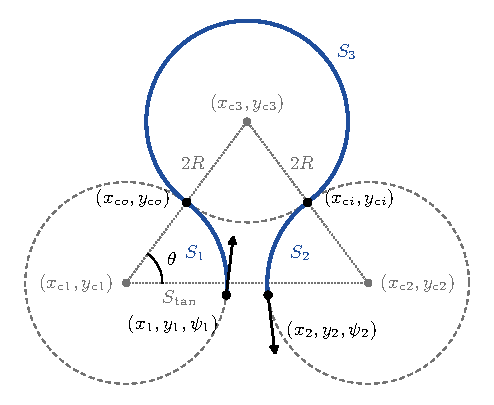
\includegraphics[width=0.6\textwidth]{fig_ccc.pdf}
  \caption{An LRL path, drawn by \code{dubins\_path.py} with $R = 5$\,m. The outer centres are $\Stan = 12$\,m apart,
  so $\theta = \cos^{-1}(12/20) = 53.13^\circ$. The lengths are $S_1 = S_2 = 5.24$\,m and
  $S_3 = R(\pi + 2\theta) = 24.98$\,m. For these poses LRL is the shortest of the six turn types.}
  \label{fig:ccc}
\end{figure}

Here $\sigma_1 = \sigma_2$, and the middle circle, of direction $-\sigma_1$, touches both outer circles, so its centre
is $2R$ from each of theirs. Such a circle exists only if
\begin{equation}
  \Stan \le 4R.
  \label{eq:ccc-exists}
\end{equation}
The three centres form a triangle with sides $2R$, $2R$ and $\Stan$ (Figure~\ref{fig:ccc}). Its angle at
$(x_{c1}, y_{c1})$ is
\begin{equation}
  \theta = \cos^{-1}\!\left(\frac{\Stan}{4R}\right), \qquad 0 \le \theta \le \frac{\pi}{2},
  \label{eq:theta}
\end{equation}
and the centre of the middle circle is
\begin{equation}
  x_{c3} = x_{c1} + 2R\cos(\psi_L + \sigma_1\theta), \qquad
  y_{c3} = y_{c1} + 2R\sin(\psi_L + \sigma_1\theta).
  \label{eq:c3}
\end{equation}
Two circles touch halfway between their centres, and there the sink's heading is at a right angle to the line joining
the centres. This gives the headings at the cut-out and the cut-in point:
\begin{equation}
  \psi_{co} = \psi_L + \sigma_1\Bigl(\theta + \frac{\pi}{2}\Bigr), \qquad
  \psi_{ci} = \psi_L - \sigma_1\Bigl(\theta + \frac{\pi}{2}\Bigr).
  \label{eq:ccc-headings}
\end{equation}
By eq.~\eqref{eq:turn}, the arc lengths are
\begin{equation}
  \begin{aligned}
  S_1 &= R\,\Turn_{\sigma_1}(\psi_1, \psi_{co}) = R\,\bigl[\sigma_1(\psi_{co} - \psi_1) \bmod 2\pi\bigr],\\
  S_3 &= R\,\Turn_{-\sigma_1}(\psi_{co}, \psi_{ci}) = R\,\bigl[-\sigma_1(\psi_{ci} - \psi_{co}) \bmod 2\pi\bigr]
       = R\,\bigl[(\pi + 2\theta) \bmod 2\pi\bigr],\\
  S_2 &= R\,\Turn_{\sigma_2}(\psi_{ci}, \psi_2) = R\,\bigl[\sigma_2(\psi_2 - \psi_{ci}) \bmod 2\pi\bigr],
  \end{aligned}
  \label{eq:ccc-arcs}
\end{equation}
and the total path distance is
\begin{equation}
  \boxed{\Spath = S_1 + S_3 + S_2.}
  \label{eq:ccc-total}
\end{equation}
Because $0 \le \theta \le \pi/2$, the middle arc is $S_3 = R(\pi + 2\theta)$, at least half a circle, whenever
$\Stan > 0$. When $\Stan = 0$ the two outer circles coincide, $\theta = \pi/2$, and the code gives $S_3 = 0$ instead
of $2\pi R$: the path then stays on the one circle. Of the two circles that touch both outer circles, the code always
uses the one on side $\sigma_1$ of the line of centres, whose arc is the longer one, $S_3 \ge \pi R$. Only that one
can belong to a shortest path [1]. If $\Stan > 4R$, the code returns $S_1 = S_3 = S_2 = \infty$.

\subsection{When Each Turn Type Exists}

\begin{table}[!htb]
\centering
\small
\caption{Existence of the six turn types. $\Stan$ is computed with the centres of that turn type.}
\label{tab:exists}
\begin{tabular}{@{}l l l@{}}
\toprule
Turn type & Middle part & Exists when \\
\midrule
LSL, RSR & straight, $\dcoci = \Stan$ & always \\
LSR, RSL & straight, $\dcoci = \sqrt{\Stan^2 - 4R^2}$ & $\Stan \ge 2R$ \\
RLR, LRL & arc, $S_3 = R(\pi + 2\theta)$ & $\Stan \le 4R$ \\
\bottomrule
\end{tabular}
\end{table}

\section{Choosing the Path}
\label{sec:choose}

\begin{figure}[t]
  \centering
  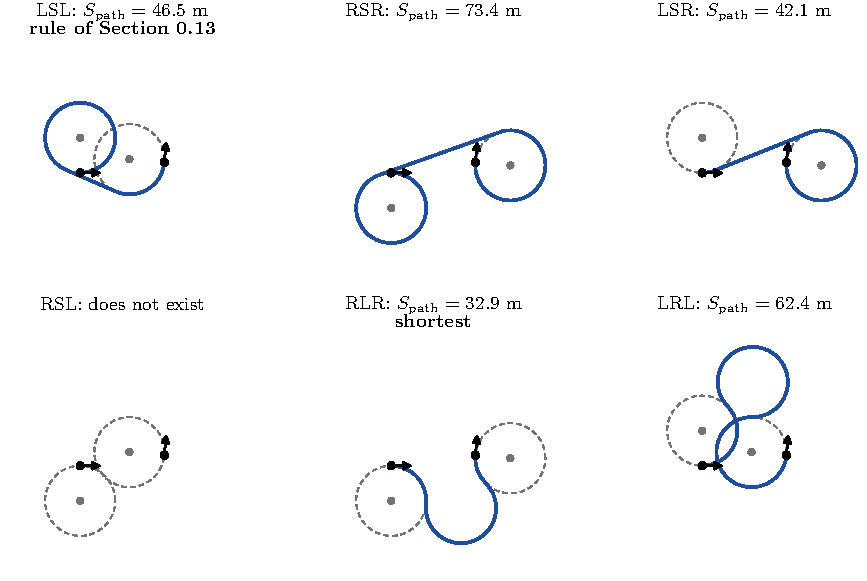
\includegraphics[width=\textwidth]{fig_six_types.pdf}
  \caption{The six turn types from $(0, 0, 0^\circ)$ to $(12, 1.5, 85^\circ)$ with $R = 5$\,m, drawn by
  \code{dubins\_path.py}. RSL does not exist: its circles are $\Stan = 9.87$\,m apart, less than $2R$. Here
  $cp_1 = 1.5 > 0$ and $cp_2 = 11.82 > 0$, so the rule of Section~0.13 picks LSL; its circles are 7.66\,m apart, below
  $2R$, so it stays LSL. LSL is 46.5\,m long, 41\,\% longer than the shortest path, RLR (32.9\,m).}
  \label{fig:six}
\end{figure}

For a turn type $T$, let $\Spath(T)$ be its total length from eq.~\eqref{eq:csc-total} or eq.~\eqref{eq:ccc-total},
with $\Spath(T) = \infty$ if $T$ does not exist. The function \code{findDubinsPath} chooses the turn type in one of two
ways, set by \code{p["dubins\_method"]} in \code{config.py}.

\paragraph{\code{"shortest"}} (the default). Compute all six and keep the shortest:
\begin{equation}
  T^{*} = \operatorname*{arg\,min}_{T} \Spath(T), \qquad T \in \{\TT{LSL}, \TT{RSR}, \TT{LSR}, \TT{RSL}, \TT{RLR}, \TT{LRL}\}.
  \label{eq:shortest}
\end{equation}
A tie goes to the turn type that comes first in the order LSL, RSR, LSR, RSL, RLR, LRL. Dubins proved that a shortest
path with turn radius at least $R$ is of type CSC or CCC, with the middle arc of a CCC path longer than $\pi R$ [1].
For each turn type the formulas of Section~\ref{sec:lengths} give the only such candidate (with every arc shorter than a
full circle), so $T^{*}$ is the shortest path.

\paragraph{\code{"pdf"}.} Take the turn type $T_{\mathrm{rule}}$ of Section~\ref{sec:rule}, unless it does not exist:
\begin{equation}
  T = \begin{cases}
        T_{\mathrm{rule}} & \text{if } \Spath(T_{\mathrm{rule}}) < \infty,\\
        T^{*}             & \text{otherwise.}
      \end{cases}
  \label{eq:pdf-choice}
\end{equation}
Section~0.13 does not say what to do when $T_{\mathrm{rule}}$ does not exist; the code uses the shortest turn type that
does. The rule does not always give the shortest path (Figure~\ref{fig:six}): the signs of $cp_1$ and $cp_2$ only say
on which side the end point and the end heading lie, and a CCC curve, which can exist up to $\Stan = 4R$ and can be the
shortest above $3R$, is tried only for $2R \le \Stan < 3R$.

\paragraph{Lengths only} (\code{returnPathDistances}). The heading search of \code{trajectory.py} needs only the
length, for many headings at once. With start headings $\psi_1^{(i)}$ and end headings $\psi_2^{(j)}$ it computes the
table
\begin{equation}
  L_{ij} = \Spath\bigl(T_{ij}\bigr) \quad\text{for the poses } \bigl(x_1, y_1, \psi_1^{(i)}\bigr),\ \bigl(x_2, y_2, \psi_2^{(j)}\bigr),
  \label{eq:table}
\end{equation}
where $T_{ij}$ is chosen by eq.~\eqref{eq:shortest} or eq.~\eqref{eq:pdf-choice}, as in \code{findDubinsPath}.

\section{The Points of the Path}

These formulas are in \code{calculateCSCTrajectory}, \code{calculateCCCTrajectory} and \code{returnDubinsPath}.

\paragraph{Spacing.} The points are placed at the distances along the path
\begin{equation}
  s_j = j\,\Delta s, \quad j = 0, 1, \ldots, J - 1, \qquad J = \Bigl\lceil \frac{\Spath}{\Delta s} \Bigr\rceil,
  \qquad\text{and}\qquad s_J = \Spath,
  \label{eq:spacing}
\end{equation}
so consecutive points are $\Delta s$ apart along the path on every part, except that the end point is always
included. The default is $\Delta s = 0.25$\,m. A part that starts at distance $a$ and has length $\ell$ gets the
points with $a \le s_j < a + \ell$, at the distance $s_j - a$ from its own start.

\subsection{CSC Trajectory}

\paragraph{First circular arc: Cut-out point.} For $0 \le s < S_1$ the point is given by eq.~\eqref{eq:arc} from
$(x_1, y_1, \psi_1)$ with direction $\sigma_1$. At $s = S_1$, with $\alpha_1 = S_1 / R$, it reaches the cut-out point
\begin{equation}
  \boxed{
  \begin{aligned}
  x_{co} &= \cos\alpha_1\,(x_1 - x_{c1}) - \sigma_1 \sin\alpha_1\,(y_1 - y_{c1}) + x_{c1},\\
  y_{co} &= \sigma_1 \sin\alpha_1\,(x_1 - x_{c1}) + \cos\alpha_1\,(y_1 - y_{c1}) + y_{c1},
  \end{aligned}}
  \label{eq:cutout}
\end{equation}
with heading, by eq.~\eqref{eq:arc-heading},
\begin{equation}
  \psi_D = \psi_1 + \sigma_1 \frac{S_1}{R},
  \label{eq:psiD-traj}
\end{equation}
which is the $\psi_D$ of eq.~\eqref{eq:csc-same} or eq.~\eqref{eq:csc-cross} up to a multiple of $2\pi$.

\paragraph{Straight trajectory.} The unit vector of the straight part is
\begin{equation}
  \hat{u} = \begin{bmatrix} \cos\psi_D \\ \sin\psi_D \end{bmatrix},
  \label{eq:uhat}
\end{equation}
and for $S_1 \le s < S_1 + \dcoci$ the point is
\begin{equation}
  \begin{bmatrix} x(s) \\ y(s) \end{bmatrix} = \begin{bmatrix} x_{co} \\ y_{co} \end{bmatrix} + (s - S_1)\,\hat{u}.
  \label{eq:straight}
\end{equation}
The straight part ends at the cut-in point
\begin{equation}
  \boxed{
  \begin{bmatrix} x_{ci} \\ y_{ci} \end{bmatrix} = \begin{bmatrix} x_{co} \\ y_{co} \end{bmatrix} + \dcoci\,\hat{u}.}
  \label{eq:cutin}
\end{equation}

\paragraph{Second circular arc.} For $S_1 + \dcoci \le s < \Spath$ the point is given by eq.~\eqref{eq:arc} from
$(x_{ci}, y_{ci}, \psi_D)$ with direction $\sigma_2$ and distance $s - S_1 - \dcoci$; by eq.~\eqref{eq:centre} the
centre of this circle is $(x_{c2}, y_{c2})$. The end point, at distance $S_2$ on this arc, is $(x_2, y_2)$, and the
final heading is
\begin{equation}
  \psi_T = \psi_D + \sigma_2 \frac{S_2}{R} \equiv \psi_2 \pmod{2\pi}.
  \label{eq:csc-end}
\end{equation}

\paragraph{Comparison with Section~0.13.} Section~0.13 finds the cut-in point by turning the end point back through
$\alpha_2 = S_2 / R$ about $(x_{c2}, y_{c2})$,
\begin{equation}
  \begin{aligned}
  x_{ci} &= \cos\alpha_2\,(x_2 - x_{c2}) + \sigma_2 \sin\alpha_2\,(y_2 - y_{c2}) + x_{c2},\\
  y_{ci} &= -\sigma_2 \sin\alpha_2\,(x_2 - x_{c2}) + \cos\alpha_2\,(y_2 - y_{c2}) + y_{c2},
  \end{aligned}
  \label{eq:cutin-back}
\end{equation}
and takes $\hat{u}$ as the unit vector from the cut-out to the cut-in point. The code instead goes forward with
eqs.~\eqref{eq:uhat} and \eqref{eq:cutin}, so each part starts exactly where the previous one ended. Both give the
same point: the two differ by less than $10^{-13}$\,m in the check described at the start.

\subsection{CCC Trajectory}

\paragraph{First circular arc.} As in the CSC case: eq.~\eqref{eq:arc} from $(x_1, y_1, \psi_1)$ with direction
$\sigma_1$ for $0 \le s < S_1$, reaching the cut-out point of eq.~\eqref{eq:cutout} with $S_1$ from
eq.~\eqref{eq:ccc-arcs}, and the heading $\psi_T = \psi_1 + \sigma_1 S_1 / R \equiv \psi_{co}$.

\paragraph{Middle circular arc.} For $S_1 \le s < S_1 + S_3$ the point is given by eq.~\eqref{eq:arc} from
$(x_{co}, y_{co}, \psi_T)$ with direction $-\sigma_1$ and distance $s - S_1$. By eqs.~\eqref{eq:centre} and
\eqref{eq:ccc-headings} the centre of this circle is
\[
  x_{co} + R\cos\Bigl(\psi_{co} - \sigma_1\frac{\pi}{2}\Bigr) = x_{c1} + 2R\cos(\psi_L + \sigma_1\theta), \qquad
  y_{co} + R\sin\Bigl(\psi_{co} - \sigma_1\frac{\pi}{2}\Bigr) = y_{c1} + 2R\sin(\psi_L + \sigma_1\theta),
\]
which is the centre $(x_{c3}, y_{c3})$ of eq.~\eqref{eq:c3}. At distance $S_3$ it reaches the cut-in point, with
heading $\psi_T \leftarrow \psi_T - \sigma_1 S_3 / R \equiv \psi_{ci}$.

\paragraph{Last circular arc.} For $S_1 + S_3 \le s < \Spath$ the point is given by eq.~\eqref{eq:arc} from
$(x_{ci}, y_{ci}, \psi_T)$ with direction $\sigma_2$ and distance $s - S_1 - S_3$. It ends at $(x_2, y_2)$ with heading
$\psi_T \leftarrow \psi_T + \sigma_2 S_2 / R \equiv \psi_2 \pmod{2\pi}$.

\paragraph{Closed forms.} The cut-out and cut-in points computed this way are the touching points of the circles,
halfway between their centres, as written in Section~0.13.2:
\begin{equation}
  \begin{aligned}
  x_{co} &= x_{c1} + R\cos(\psi_L + \sigma_1\theta), & y_{co} &= y_{c1} + R\sin(\psi_L + \sigma_1\theta),\\
  x_{ci} &= x_{c2} - R\cos(\psi_L - \sigma_1\theta), & y_{ci} &= y_{c2} - R\sin(\psi_L - \sigma_1\theta).
  \end{aligned}
  \label{eq:ccc-points}
\end{equation}

\subsection{Output}

\code{returnDubinsPath} returns
\begin{equation}
  \bigl(\xtraj,\ \ytraj,\ \Spath,\ \straj\bigr),
  \label{eq:output}
\end{equation}
where
\[
  \xtraj = \bigl(x(s_0), \ldots, x(s_J)\bigr), \qquad
  \ytraj = \bigl(y(s_0), \ldots, y(s_J)\bigr), \qquad
  \straj = (s_0, \ldots, s_J).
\]
At the constant speed of eq.~\eqref{eq:kinematics}, the sink reaches point $j$ at time $s_j / v$ after the start of
the path. These times are what \code{trajectory.py} uses to place the sink on the shared timeline.

\section{What the Construction Guarantees}

\begin{itemize}
  \item \textbf{No corners.} Each part starts at the point and with the heading at which the previous part ended
        (eqs.~\eqref{eq:arc}, \eqref{eq:arc-heading}, \eqref{eq:psiD-traj} and \eqref{eq:cutin}), so the position and
        the heading are continuous along the whole path.
  \item \textbf{Turning radius.} Every arc has radius exactly $R$ and the straight part has none, so the path never
        turns tighter than $R$. Every part has a length of at least 0, by eq.~\eqref{eq:turn}.
  \item \textbf{End pose.} The last point is $(x_2, y_2)$ and the final heading is $\psi_2$ up to a multiple of
        $2\pi$, apart from rounding: at most $8 \times 10^{-14}$\,m and $4 \times 10^{-15}$\,rad in the check described
        at the start. The test \code{test\_dubins\_every\_turn\_type\_reaches\_the\_target\_smoothly} checks this for
        every turn type.
  \item \textbf{Shortest.} With \code{"shortest"} the path is the shortest path with turning radius at least $R$
        (Section~\ref{sec:choose}). With \code{"pdf"} it can be longer (Figure~\ref{fig:six}).
\end{itemize}

\section{Numerical Safeguards}

Table~\ref{tab:guards} lists every tolerance and clamp in the code. None of them changes a result by more than
rounding; they stop a rounding error from deciding whether a path exists, or from producing a full circle or an
invalid $\sin^{-1}$, $\cos^{-1}$ or square root.

\begin{table}[!htb]
\centering
\small
\caption{Tolerances and clamps in \code{dubins\_path.py}.}
\label{tab:guards}
\begin{tabular}{@{}l l l@{}}
\toprule
Where & What the code does & Why \\
\midrule
\code{turnAngle} & $\Turn > 2\pi - 10^{-6} \Rightarrow \Turn = 0$ & ``no turn'' must not become a full circle \\
RSR, LSL & $\Stan < 10^{-9} \Rightarrow \psi_D = \psi_1$ & $\psi_L$ means nothing when the circles coincide \\
LSR, RSL & exists if $\Stan \ge 2R - 10^{-9}$ & circles that only just touch count \\
LSR, RSL & $\beta = \sin^{-1}\bigl(\min\{2R / \max(\Stan, 10^{-9}),\, 1\}\bigr)$ & no division by zero; $\sin^{-1}$ defined \\
LSR, RSL & $\dcoci = \sqrt{\max(\Stan^2 - 4R^2,\, 0)}$ & no square root of a negative number \\
RLR, LRL & exists if $\Stan \le 4R + 10^{-9}$ & circles that only just touch count \\
RLR, LRL & $\theta = \cos^{-1}\bigl(\min\{\Stan / 4R,\, 1\}\bigr)$ & $\cos^{-1}$ defined \\
all & a turn type that does not exist has length $\infty$ & it is never the shortest \\
\bottomrule
\end{tabular}
\end{table}

\section{Relation to Section 0.13 of the Paper}

Table~\ref{tab:paper} compares the original text of Section~0.13 with the code. The blue additions marked in
Section~0.13 of \code{Dubins\_TSP.pdf} state the formulas of the right-hand column.

\begin{table}[!htb]
\centering
\small
\caption{Section 0.13 (original text) and \code{dubins\_path.py}.}
\label{tab:paper}
\begin{tabular}{@{}>{\raggedright}p{0.2\textwidth} >{\raggedright}p{0.33\textwidth} >{\raggedright\arraybackslash}p{0.38\textwidth}@{}}
\toprule
Topic & Section 0.13 & \code{dubins\_path.py} \\
\midrule
Choice of turn type & rule of eq.~\eqref{eq:rule} only & rule (\code{"pdf"}) or shortest of six (\code{"shortest"}, default), eqs.~\eqref{eq:shortest}--\eqref{eq:pdf-choice} \\
$cp_2 = 0$ & not covered & treated like $cp_2 > 0$ \\
$u_2$ & unit vector & not divided by its length \\
Which types become CCC & ``if $2R \le \Stan < 3R$'' for every type & only RSR and LSL, eq.~\eqref{eq:rule-ccc} \\
$\psi_L$ & $(y_{c2} - y_{c1}) / (x_{c2} - x_{c1})$ & $\operatorname{atan2}$, eq.~\eqref{eq:psiL} \\
$\psi_D$ for LSR, RSL & $\psi_L \pm \tan^{-1}(2R / \Stan)$ & $\psi_L \pm \sin^{-1}(2R / \Stan)$, eq.~\eqref{eq:csc-cross} \\
Arcs & steps of $\Delta\psi = 0.05$ until $|\psi_T - \psi_D| \le 0.1$ & exact angle, eqs.~\eqref{eq:turn}, \eqref{eq:csc-arcs}, \eqref{eq:ccc-arcs} \\
Turn type that does not exist & not covered & shortest turn type that exists \\
CCC geometry & not given & eqs.~\eqref{eq:theta}--\eqref{eq:ccc-total}, \eqref{eq:ccc-points} \\
Spacing of points & 3 on the straight part only & $\Delta s$ on every part, eq.~\eqref{eq:spacing} \\
\bottomrule
\end{tabular}
\end{table}

\section*{Reference}

[1] L. E. Dubins, ``On curves of minimal length with a constraint on average curvature, and with prescribed initial
and terminal positions and tangents,'' American Journal of Mathematics, vol.~79, no.~3, pp.~497--516, 1957.

\end{document}
